	\chapter{Incremental Self Organizing Maps based Collaborative Clustering}
\label{ccisom}

\minitoc{}
\newpage

    \section{Introduction}

    Collaborative Clustering makes it possible for several independant views to collaborate. An incremental method for this problem, in which data are continuously added to each view through time, would make possible for a set of views to collaborate all along their existence, and not only at a fixed point in time. Thus, the different collaboration could follow a possible changement in data distribution through time. To clarify a detail which differenciate online and incremental methods, unlike the former, the latter are allowed to store a batch of data when they arrive, making it possible to work with batches instead of just singletons.
	
    The elaboration of such a method presents several challenges. As presented in~\ref{sec:soa_cc}, Collaborative Clustering relies on prototype based clustering, thus reducing the number of available clustering algorithms. The second one lies in the adaptation of the collaborative update rules depending on the chosen clustering method. In this chapter we try to address theses challenges by focusing on the case of SOM.\@
	
    The work presented here consists in an incremental SOM-based Collaborative Clustering method without topological modification of the SOM and which is robust to a possible data distribution evolution. The key component of this approach lies in the modification of the temperature function of the SOM which does not depend on time anymore.
	
    The rest of this chapter is organized as follows: our approach on incremental SOM and its application to Collaborative Clustering is presented in Section~\ref{ccisom}, followed by the experimental results presented in Section~\ref{experiments}. Eventually, a further analysis of our method is presented (easymotion-prefix) in Section~\ref{conclusion}.
	
	\section{Incremental Collaborative Clustering}
    Incremental SOM have already been studied in the litterature. However, all the presented solutions are based on topological modifications of the map~\cite{deng2000esom,paplinski2012incremental}, and this kind of modifications are not compatible with the Collaborative Clustering update rules. Indeed, the Collaborative Clustering paradigm supposes that each dataset describes its data by the same number of prototypes to allow comparisons between several views and to keep topological mapping between each pair of views. In our case, the prototypes correspond to the neurons of the SOM, and as such without modification of the algorithm, the topology of each SOM has to be fixed during the initialization of the algorithm. Another problem encountered in general with incremental clustering is the possibility for the algorithms to answer changes in the data distribution through time. If the data distribution evolves, one has to be sure that the prototypes will follow the distribution of the most recent batches.
	
	\section{Incremental SOM}
\label{sectionisom}
	In our incremental version of SOM, we consider that the data are arriving all along the experiment. Therefore we assume that at each moment the model only knows the batch $B$ of the $N_{batch}$ last samples that have appeared during the learning.
	Our method here presents a variation of the original temperature function which aims at avoiding the dependence between the temperature and the time. This is motivated by the incremental aspect of the subject, for which it is not possible to define a time limit $t_{\max}$ at which the algorithm will end. In order to make the SOM responsive to the arrival of new data, a new function $\widetilde{\lambda}$ is defined by:
	
	\begin{equation}
	\widetilde{\lambda}(B, W) = \frac{1}{N_{batch}}\sum_{i=1}^{N_{batch}}\|x_i - \chi(x_i)\|_2
	\end{equation}
	
	With $B \subset X$ the batch currently used and with $|B|=N_{batch}$. This $\widetilde{\lambda}$ function is then capped between $\lambda_{\min}$ and $\lambda_{\max}$ in order to avoid extreme modifications of the SOM.\@ This definition of the temperature function allows the SOM to be more responsive to novelty encountered in the batch. If the elements of a batch are far from the current neurons, the whole map would need to be adjusted to the new distribution of the sample, and this case is empirically achieved for high values of $\widetilde{\lambda}$. On the opposite, if the samples are near the current centroids, the map only needs some adjustments in order to better match the sample distribution. This case is achieved for low values of $\widetilde{\lambda}$. To clarify notations, the neighboring function which is defined by $\widetilde{\lambda}$ will be named $\widetilde{K}$.
	
	\section{Adaptation to Collaborative Clustering}
	In this paper, we only consider the case of horizontal Collaborative Clustering as defined in~\cite{ghassany2012collaborative}. For the rest of this paper, we consider datasets $\{X[i] | i \in 1..P\}$ containing the same set of objects described in different spaces, with P models (in our case SOM) being trained to represent each view separately. To clarify notation, $W^{m \in \{1..P\}}$ names the $m$-th model created using the $m$-th dataset. The point of Collaborative Clustering is to make those models collaborate in order to reveal common structures among them. The main hypothesis that is made here is if an observation from the $i$-th dataset belongs to the $j$-th neuron of the $i$-th model, then the same observation in the $i'$-th model will also belong to its $j$-th neuron or to its neighborhood. In other words, \textit{equivalent neurons from different maps should capture the same observations}~\cite{ghassany2012collaborative}.
		
	In order to adapt the original criterion to the incremental version of Collaborative Clustering, we use an approximation of this criterion using the kernel function $\widetilde{K}$ defined in Section~\ref{sectionisom} and where the distance are summed over the current batch instead of over the whole dataset:
	
		\begin{equation}
\label{criterion}
		\widetilde{R}^m(\chi, \omega) = \widetilde{R}_{Local}(W) + \widetilde{R}_{Collab}(W)
		\end{equation}
		
		\begin{equation}
\label{criterion2}
		\widetilde{R}_{Local}(W) = \alpha_m\sum_{i=1}^{N_{batch}}\sum_{j=1}^{|W|}\widetilde{K}^m_{j, \chi(x_i)}\|x_i^k - \omega_j^k\|^2
		\end{equation}
		
		\begin{equation}
        \widetilde{R}_{Collab} = \sum_{m'=1, m'\neq m}^{P}\beta_m^{m'}\sum_{i=1}^{N_{batch}}\sum_{j=1}^{|W|}{(\widetilde{K}^m_{j, \chi(x_i)} - \widetilde{K}^{m'}_{j, \chi(x_i)})}^2  \|x_i^m - \omega_j^m\|^2
		\end{equation}
		
		\begin{algorithm}[H]
			\caption{Incremental horizontal Collaborative Clustering}
\label{alg1}
				Set the collaboration matrix $\{\alpha_{i,j}\}$\\
			    \While{Experiment going on}{
                    \If{new sample appears}{
                        Update batch as a FIFO stack of samples\\
                        \textbf{1. Local Step}\\
                        \ForAll{$m \in 1..P$}{
                            Update prototypes of $W^m$ with one pass of incremental SOM
                        }
                        \textbf{2. Collaboration Step}\\
                        \For{$m \in {1..P}$}{
                            \For{$\omega \in W^m$}{
                            $\omega = \omega + \frac{\sum_{i=1}^{N_{batch}}\widetilde{K}^m_{j,\chi(x_i^m)}\Delta_i^m + \sum_{m'=1, m'\neq m}^{P}\sum_{i=1}^{N}\alpha_m L_{ij}\Delta_i^m}{\sum_{i=1}^{N_{batch}}\widetilde{K}^m_{j,\chi(x_i^m)} + \sum_{m'=1, m'\neq m}^{P}\sum_{i=1}^{N}\alpha_m L_{ij}}$\\
                        with $L_{ij} = {(\widetilde{K}^m_{j, \chi{x_i}} - \widetilde{K}^{m'}_{j, \chi{x_i}})}^2$ and $\Delta_i^m = (x_i^m - \omega)$
                            }
                        }
                    }
				}
		\end{algorithm}
		
	With $\alpha$ and $\beta$ being defined as the collaboration coefficients, which in our cases are fixed by the user at the beginning of the experiments. Each $\alpha$ and $\beta$ defines the comparative weights of the local and collaboratives terms in relation to each other.
	
	A summary of the incremental horizontal Collaborative Clustering can be found in Alg.~\ref{alg1}.
	
	It is interesting to note that a lot of computation time may be avoided by performing the local step only during the first few steps of the algorithm. The first local steps help to improve the final quality of the clustering in terms of mean neurons to samples distance, whereas additional steps do not change much the final results.
	
	\section{Experimental Results}
\label{experiments}
	
	\subsection{Datasets and quality measures}
    To evaluate the method presented in this paper, we have tested them on four different datasets found on the UCI website~\cite{uci}: Spam Base, Waveform, Wisconsin Diagnostic Breast Cancer (WDBC) and Isolet. Their respective descriptions can be found in Appendix~\ref{sec:app-datasets}.

	During our experiments, each of those datasets has been normalized and divided in 3 views each containing a third of the original variables. We suppose here that one has enough information on each variable to allow its normalization at the time it appears, for example by knowing its bounds. Each view will stand for an individual ``site'' which will collaborate with its peers.
	
	The quality measures used during those experiments are the quantization error and the purity index commonly used to analyze SOM.\@
	
	The quantization error can be defined in our case by the following expression:
	\begin{equation}
	qe = \frac{1}{N_{batch}}\sum_{i=1}^{N_{batch}}\|x_i - \omega_{\chi(x_i)}\|^2
	\end{equation}
	
	The purity of a neuron is defined by the proportion of the most represented class, and the purity of a map is equal to the average purity of its neurons. 
		
	\subsection{Experiments}
	In this section we present the results obtained on the four datasets. For these experiments, a 10$\times$10 SOM has been used, with $\lambda_{\min}=0.3$, $\lambda_{\max}=3$, $\epsilon=0.5$ (while it is usually time-dependent for classical SOM), $N_{batch}=10$ and the local step of Collaborative Clustering has been performed for the first 10 batches. The models have been trained using only the 30 first batches in order to test the early convergence of the model and because it appears that the results do not change a lot on the long term. The methods have been coded in R v3.2.3.
	
	\begin{table}[!h]
		\caption{Mean quantization errors on each database. ISOM stands for Incremental SOM and ICollaborative Clustering stands for Incremental Collaborative Clustering. Bold numbers are the lowest ones for each line.}
		\begin{center}
\begin{tabular}{cccc}
                           & View & Incremental SOM & \begin{tabular}[c]{@{}c@{}}Incremental\\ Collaborative Clustering\end{tabular} \\ \midrule
\multirow{3}{*}{Spam Base} & 1    & 0.31            & \textbf{0.26}                                                                  \\
                           & 2    & \textbf{0.18}   & 0.19                                                                           \\
                           & 3    & 0.18            & \textbf{0.16}                                                                  \\ \midrule
\multirow{3}{*}{Waveform}  & 1    & \textbf{0.18}   & 0.23                                                                           \\
                           & 2    & \textbf{0.17}   & 0.19                                                                           \\
                           & 3    & \textbf{0.24}   & 0.30                                                                           \\ \midrule
\multirow{3}{*}{WDBC}      & 1    & \textbf{0.19}   & 0.19                                                                           \\
                           & 2    & \textbf{0.16}   & 0.19                                                                           \\
                           & 3    & 0.20            & \textbf{0.16}                                                                  \\ \midrule
\multirow{3}{*}{Isolet}    & 1    & 2.15            & \textbf{1.27}                                                                  \\
                           & 2    & 2.84            & \textbf{1.38}                                                                  \\
                           & 3    & 2.85            & \textbf{1.37}                                                                 \\ \midrule
\end{tabular}
		\end{center}
\label{tab:tab1}
	\end{table}
	
	The purities of the maps can be seen on Fig.~\ref{img1}, Fig.~\ref{img2} and Fig.~\ref{img3}. For the sake of clarity, only the results for the Isolet dataset are presented here. It appears that Collaborative Clustering improves the purity of the maps even if it makes it less stable than the incremental SOM.\@ The terms stable and unstable refers here to the standard deviation of the purities through time, which is higher in the case of Collaborative Clustering.\@ This instability could be caused by the batch learning. The results of the learning phase depends on the incoming data: if one specific class is more represented than the others in a batch (which is more prone to happen if the batch is small), the neurons updates for this step will focus on this class specifically, and in the end it might hurt the next phases because of the bias acquired by the model for this specific class. An increase of the instability of the purities proportionally to the decrease of the batch size can be seen by comparing Fig.~\ref{img1},~\ref{img2} and~\ref{img3} to Fig.~\ref{img4},~\ref{img5} and~\ref{img6}, where we have set $N_{batch}=3$. It is possible that the collaborative part of Eq.~\ref{criterion} makes the centroids move from the local solution minimizing Eq.~\ref{criterion2}: the collaborative SOM makes the centroid move toward a global solution rather than toward a local one. Concerning the quantization errors presented in Table~\ref{tab:tab1}, they all stay in an acceptable range considering that the data are scaled before the training. The case of the Isolet dataset is special because there are many more features than in the other datasets, and the database is sparser, point which may lower the performances of each local model depending on the distribution of features. Otherwise, it appears that the errors are always close to each other with a small advantage for the incremental SOM.\@ 
	
				\begin{figure}[!h]
					\centering
                    \subfloat[$N_{batch}=10$, View 1]{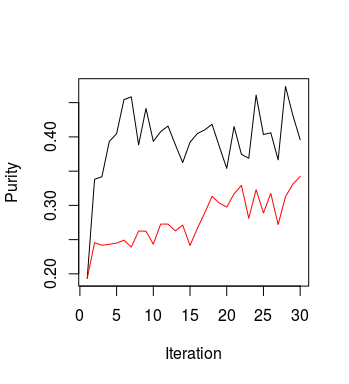
\includegraphics[width=0.33\textwidth, trim= 0 0.5cm 1cm 2cm, clip]{img/11.png}\label{img1}}
                    \subfloat[$N_{batch}=10$, View 2]{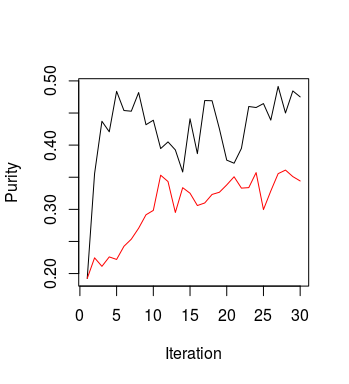
\includegraphics[width=0.33\textwidth, trim= 0 0.5cm 1cm 1.73cm, clip]{img/22.png}\label{img2}}
                    \subfloat[$N_{batch}=10$, View 3]{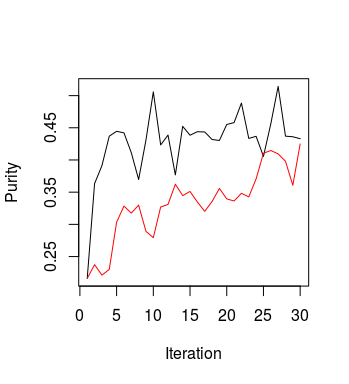
\includegraphics[width=0.33\textwidth, trim= 0 0.5cm 1cm 2cm, clip]{img/33.png}\label{img3}}\\
                    \subfloat[$N_{batch}=3$, View 1]{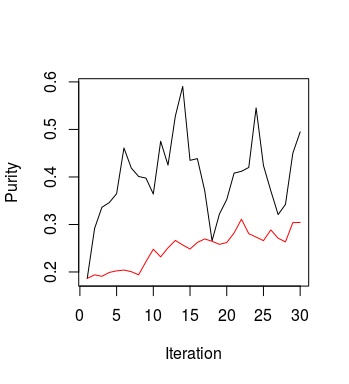
\includegraphics[width=0.33\textwidth, trim= 0 0.5cm 1cm 1.9cm, clip]{img/p1.png}\label{img4}}
                    \subfloat[$N_{batch}=3$, View 2]{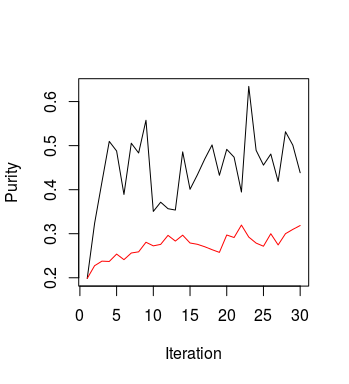
\includegraphics[width=0.33\textwidth, trim= 0 0.5cm 1cm 2cm, clip]{img/p2.png}\label{img5}}
                    \subfloat[$N_{batch}=3$, View 3]{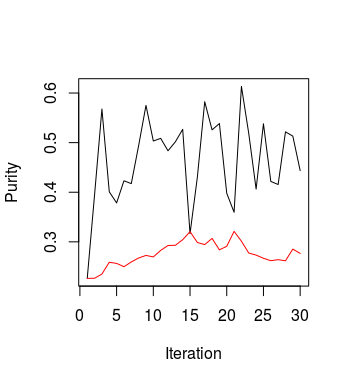
\includegraphics[width=0.33\textwidth, trim= 0 0.5cm 1cm 2cm, clip]{img/p3.png}\label{img6}}
					\caption{Evolution of the purities for the Isolet database with 2 different $N_{batch}$. The red lines represent the incremental SOM whereas the black lines represent the collaborative SOM.\@ Each iteration corresponds to the arrival of a new sample}
				\end{figure}

	\section{Conclusion}
\label{conclusion}
	In this study, we proposed a methodology to perform incremental SOM without topological modifications of the map as well as the application of this method to adapt horizontal Collaborative Clustering according to the incremental constraint. Its application to vertical Collaborative Clustering is possible but has not been described in this paper. With these methods, the temperature function $\widetilde{\lambda}$, and so the neighboring function $\widetilde{K}$ of the generated maps are no longer time-dependent, and now only depend on incoming data. Knowing that, the map can be adapted to continuously incoming data. The presented methods have been tested on 4 different datasets, and the results show that the version of incremental SOM presented in this paper can be adapted to perform incremental Collaborative Clustering.\@ The influence of the parameter $N_{batch}$, namely its impact on the stability of the learning, has also been investigated.
	
	To pursue this work, we plan to investigate the methods which would allow to adapt topological modifications on SOM in the context of Collaborative Clustering.\@ Furthermore, we plan to adapt what has been presented in this research work to the GTM, which are by nature similar to SOM.\@

In the next chapter, we explore a collaboration method based on neural network and vectors rather than on scalar only. The complexity of this new method makes it possible to introduce a new use case to explore how an inter-view collaboration can be used to perform tasks different from clustering.

